\section{Membrane Dynamics}

At the heart of cellular mechanisms lies the cell membrane, which serves as far more than a simple boundary between internal and external environments. This sophisticated interface plays a crucial role in implementing ECC's principles through the precise regulation of ion flows, protein organization, and local electric fields \cite{Andersen1992}. The cell membrane emerges not as a passive barrier but as an active participant in information processing and energy management, fundamentally shaping how neural systems maintain coherent conscious states.

The phospholipid bilayer structure creates a highly organized environment where proteins can be precisely arranged and regulated to support conscious processing \cite{Goni2014}. This molecular organization enables several crucial processes that extend beyond basic cellular containment. Through careful maintenance of ion gradients and electrochemical potentials, membranes establish the fundamental conditions necessary for neural signaling and information processing. The resulting electrical properties enable neurons to maintain stable resting states while remaining capable of rapid, coordinated responses to incoming signals.

Lateral organization within the membrane reveals another layer of sophistication in cellular processing \cite{Garcia-Parajo2014}. Specialized membrane domains create distinct regions where specific proteins cluster together, enabling precise control over cellular signaling and energy management. These domains prove essential for coordinating the complex molecular interactions that underlie neural computation. Through dynamic reorganization of membrane components, cells can modify their processing capabilities while maintaining overall stability.

The membrane's role in generating and maintaining electric fields takes on particular significance for conscious processing \cite{Bezanilla2002}. Local variations in membrane potential create sophisticated patterns of field effects that influence both protein function and cellular signaling. These field effects extend beyond individual cells to shape network dynamics through ephaptic coupling and other non-synaptic mechanisms. The resulting electromagnetic properties of neural membranes contribute fundamentally to the establishment and maintenance of coherent conscious states.

The dynamic interplay between membrane structure and protein function demonstrates remarkable sophistication in neural information processing \cite{Kusumi2012}. Membrane proteins respond to changes in local electrical fields and mechanical forces, creating feedback loops that enable precise regulation of cellular activity. This intimate coupling between membrane properties and protein function enables neural systems to maintain stable processing capabilities while adapting to changing conditions.

The relationship between membrane dynamics and energy management reveals sophisticated mechanisms for maintaining conscious states \cite{Yang2019}. Through precisely regulated ion pumps and transport proteins, membranes help establish and maintain the energy gradients necessary for neural signaling. These molecular systems operate continuously to preserve the specific electrical properties required for information processing while managing cellular energy consumption.

\begin{figure}[h]
    \centering
    \includegraphics[width=0.8\textwidth]{images/membrane.png}

    \caption{Membranes have phospholipid bilayer structure.}
\end{figure}

Membrane fluidity plays a crucial role in enabling dynamic responses to neural activity \cite{Lingwood2010}. The capacity for lipids and proteins to move laterally within the membrane creates opportunities for rapid reorganization of signaling complexes and regulatory systems. This molecular mobility enables cells to adjust their processing capabilities through precise changes in protein organization and interaction. The controlled fluidity of neural membranes thus provides a fundamental mechanism for adapting to changing computational demands while maintaining functional stability.

The interface between membranes and the cytoskeleton reveals another layer of cellular regulation in conscious processing \cite{Zimmerberg2006}. Membrane proteins interact with cytoskeletal elements to create structured domains that shape both cellular architecture and signaling properties. These interactions enable precise control over protein distribution and movement while providing mechanical stability to cellular structures. The resulting membrane-cytoskeleton coupling helps establish the organized cellular domains necessary for coherent neural activity.

Lipid composition demonstrates remarkable regional variation that reflects different requirements for neural processing \cite{Yang2019}. Different areas of the membrane maintain distinct combinations of lipid species that influence local properties such as fluidity, thickness, and protein organization. These molecular variations enable cells to establish specialized domains for particular aspects of neural computation while maintaining overall membrane integrity. The precise tuning of lipid composition proves crucial for supporting the diverse functions required for conscious processing.

The role of membrane dynamics in synaptic transmission extends far beyond simple neurotransmitter release \cite{Sudhof2013}. Presynaptic membranes undergo sophisticated reorganization during vesicle fusion and recycling, while postsynaptic membranes coordinate complex patterns of receptor trafficking and clustering. These dynamic processes enable synapses to maintain reliable transmission while adapting their properties based on neural activity. The resulting synaptic plasticity depends fundamentally on precise regulation of membrane organization and dynamics.

The integration of membrane dynamics with broader patterns of neural activity reveals fundamental principles about how conscious processing emerges from cellular mechanisms \cite{Choquet2013}. Membranes serve as sophisticated interfaces that enable cells to participate in coherent network activity while maintaining their specific processing capabilities. Through precise regulation of protein organization, ion flows, and electrical properties, membranes help establish the conditions necessary for consciousness while supporting dynamic adaptation to changing demands.

The coordination between membrane organization and energy metabolism demonstrates remarkable efficiency in neural processing \cite{Goni2014}. The precise arrangement of transport proteins and metabolic machinery enables cells to maintain the energy gradients necessary for signaling while minimizing metabolic costs. This optimization reflects evolutionary refinement of membrane organization for both computational capability and energetic efficiency.

\begin{figure}[h]
    \centering
    \includegraphics[width=0.8\textwidth]{membrane.png}

    \caption{The cell membrane is where the cell receives all external information. }
\end{figure}

Perhaps most significantly, membrane dynamics demonstrate how biological systems achieve sophisticated information processing through continuous physical processes rather than discrete computational steps \cite{Sachs2010}. The fluid nature of membrane organization, coupled with precise molecular regulation, enables neural systems to maintain stable conscious states while remaining responsive to changing conditions. This understanding proves essential for explaining how consciousness emerges from biological organization rather than abstract computation.

The implications extend beyond neuroscience to fundamental questions about the nature of conscious processing \cite{Zimmerberg2006}. The remarkable sophistication of membrane dynamics suggests that consciousness requires specific forms of physical implementation that support both stability and adaptability through continuous regulation of cellular properties. This perspective challenges purely computational approaches to consciousness while suggesting new directions for developing artificial systems capable of supporting conscious-like processing.

Moving beyond membrane dynamics, we must now examine how neurotransmitter and neuromodulatory systems influence conscious processing through broad-scale regulation of neural activity \cite{Choquet2013}. These sophisticated molecular signals reshape network properties and energy dynamics across multiple spatial and temporal scales, fundamentally altering how neural circuits maintain coherent conscious states.